  \item Edycja danych klienta \\
 
 Opis słowny - przypadek użycia procesowany w momencie, gdy użytkownik (klient)
 zdecyduje się zmienić swoje dane, na przykład na skutek zmiany miejsca
 zamieszkania, adresu e-mail itp. Dane powinny być zapisane w bazie danych
 natychmiast po wprowadzeniu ich przez użytkownika i wszelkie zamówienia już
 realizowane a także te, które zostaną złożone w przyszłości
 
 \begin{longtable}{|p{5cm}|p{7cm}|}
 	\hline
	\textbf{Aktor} & Klient \\
	\hline
	\textbf{Warunki początkowe} & Klient zalogowany \\
	\hline
	\textbf{Opis przebiegu interakcji} & Zmiana danych w formularzu, zapis danych
	do bazy danych
	\\
	\hline
	\textbf{Sytuacje wyjątkowe} & Niepoprawne (nie takie same) wprowadzone hasła,
	zbyt krótkie hasło
	\\
	\hline
	\textbf{Warunki końcowe} & Poprawnie zmienione w bazie dane \\
	\hline
 \end{longtable}
 

 \item Edycja danych klienta - scenariusz główny \\
  \begin{tabularx}{\linewidth}{ c X }
  Aktor: & Klient \\
  \end{tabularx}
  \begin{enumerate}
    \item Klient uruchamia witrynę internetową sklepu
    \item Klient loguje się do systemu (tylko osoba zalogowana może zmieniać
    swoje dane)
    \item Klient edytuje wybrane pozycje ze swojego opisu (adres, numer
    telefonu itp.)
    \item W przypadku zmiany hasła klient proszony jest o podanie starego jak i
    nowego (dwukrotnie) hasła
    \item Klient zatwierdza wprowadzone zmiany
    \item System wysyła na podany przez użytkownika adres e-mail (nowy, jeśli
    to adres e-mail był jedną ze zmienianych wartości) informację o zmianie.
  \end{enumerate}
  
  
   \item Edycja danych klienta - scenariusz alternatywny - Niezgodne hasła\\
  \begin{tabularx}{\linewidth}{ c X }
  Aktor: & Klient \\
  \end{tabularx}
  \begin{enumerate}
    \item Kroki 1-4 jak w scenariuszu głównym
    \item W przypadku niezgodnych haseł system informuje użytkownika o błędzie
    wprowadzonych danych
    \item Jeśli niezgodność danych powtórzy się 3-krotnie, na e-mail użytkownika
    wysyłana jest informacja, że potencjalnie ktoś próbuje zmienić dane bez
    wiedzy upoważnionego użytkownika
  \end{enumerate}
  
  
  
  \begin{figure}[h!]
    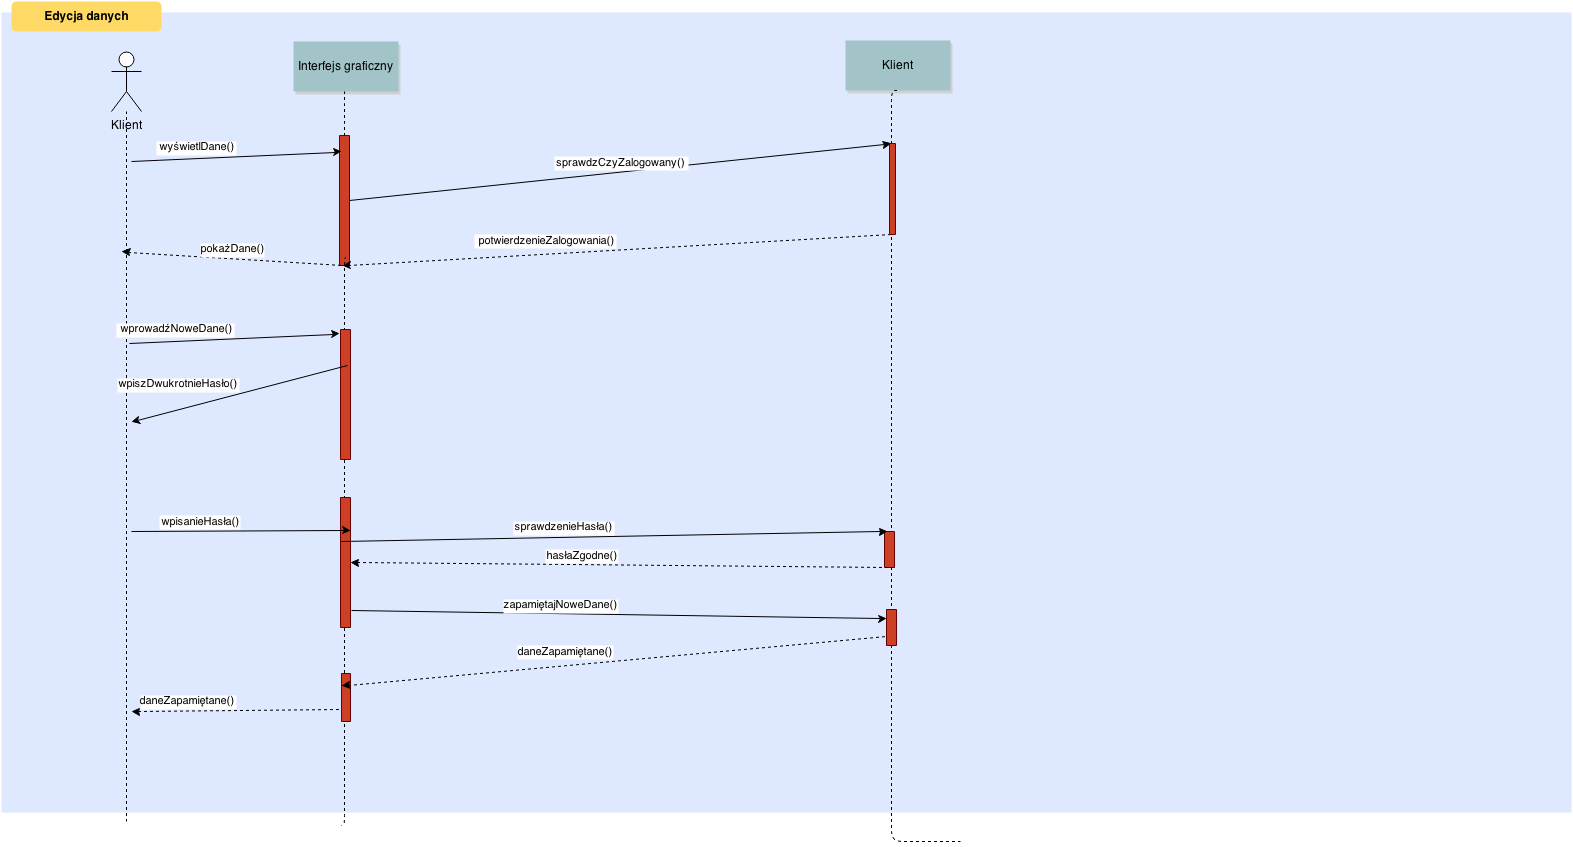
\includegraphics[width=\textwidth,
    height=0.5\textheight]{graphics/UseCase/Klient/EdycjaDanychKlientaSD.png}
  \caption{Diagram sekwencji dla przypadku użycia Edycja Danych Klienta -
  scenariusz główny}
\end{figure}